\chapter{避风港}

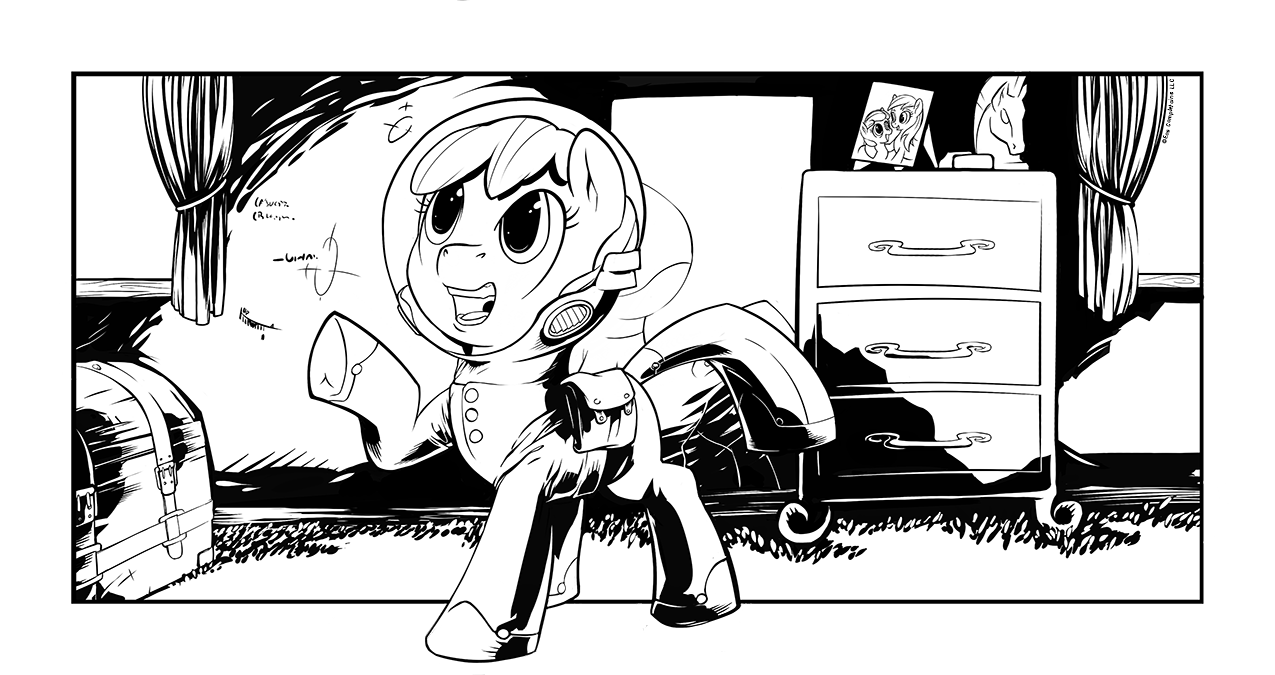
\includegraphics[width=\linewidth]{image01.png}

\begin{intro}
    你相信幽灵吗?
\end{intro}

「拜托让我们上车!防护罩要失效了!我们要来不及了!」

长长的一大队小马焦急的等在一辆飞空马车前,但是却没有看到拉车天马出现。忽然队末的一只绿色独角兽雌驹疯狂的推着马群尖叫起来。

「这不可能!不可能这样!赛蕾丝蒂娅抛弃了我们!露娜抛弃了我们!这……」

砰!

慌乱的雌驹无声地倒在了地上,所有小马齐刷刷转头看过去,卫兵正在将子弹压入霰弹枪。

「整整齐齐站成一排!排好队挨个上车!谁找麻烦我只好用致命手段了!」

一只粉色毛皮金色鬃毛的小幼驹正抬头看着就在他们头顶的中心城。巨大的闪光泡泡把整个山顶包裹住了。在泡泡里面包裹的粉色迷雾是她这辈子从来没有见过的神奇景象,完全吸引了她的注意力。

「嘿,那边的小鬼!」

一个穿着白色制服的独角兽医疗兵正在给幼驹发着防护服。她站在粉色小雌驹面前,稍微沉默了一下。

「就你自己吗?你家长哪里去了?」

幼驹对着医官微笑着。「妈妈在那上面!」她用蹄子指着中心城的闪光防护罩,防护罩现在看起来比10分钟之前已经薄了很多。「她晚餐的时候就会回来!」

士官踌躇了一下,然后对幼驹勉强一笑。「当然……她会回来的。小家伙你叫什么名字?」

「我叫快乐帕比 (Puppysmiles) !」幼驹开心地蹦蹦跳跳着。

「好的……好的……帕比,没关系……你仔细听好,穿好这件外套,不管发生什么事情,都不要脱下来,好吗?」

幼驹有些疑惑的视线在黄色的东西和白制服独角兽之间来回转了转,「好的,漂亮的大姐姐!我喜欢你!」

% TODO: 漏翻译

独角兽紧张地笑了笑,然后漂起并展开了防辐射服:那是一件柠檬黄色外套,蹄子上有几个口袋,体侧还各有一个鞍包。

「好,你要把你的蹄子放进这些洞洞里面,就像是……像是……小马舞一样!你知道小马舞吗?」

「当然!\emph{右蹄伸出去……右蹄缩回来……}」

「对对,就是这样!然后是尾巴……好了,然后让我给你密封好,最后是把这个放在你的头上……好了!」

雌驹把一个原型的玻璃头盔戴在了帕比头上,然后把两边的卡扣锁紧,把孩子安全地包在了她的防辐射服里面。

「哇塞!我看起来就像是个太空小马!就像是……像是安德洛队长一样!呜!!!」幼驹兴奋地蹦来蹦去,白色的雌驹微微松了口气,然后转头走向下一队幼驹。

快乐帕比觉得现在真开心极了。一个巨大无比的烟花爆炸了,它听起来像一个非常棒的派对礼花!城堡被超大的肥皂泡泡包着,就像是妈妈用肥皂吹出来的那样,不过要大很多很多。大家都像在大庆典之前一样走上了街头。她偷偷对自己的幸运星祈祷妈妈能够早点回家,这样今天她就能和妈妈早点在一起玩耍了。而这个超级酷的太空服更是大大的意外惊喜,看来大家都想把她打扮得漂漂亮亮的,然后……对了!现在她需要面镜子!小雌幼驹毫不犹豫地跑回家去。

\horizonline

% NOTE: 原文没有分割线

在她妈妈的卧室里面依稀听得见街上喧闹的声音,帕比站在梳妆台之前,仔细看着她的头盔,她面前出现好多奇怪的发光符号和文字。不管她看向什么那东西就会被一层奇怪的绿光笼罩,然后下面出现一些小字……可惜的是帕比认识的字不多,她妈妈还没怎么教她。

「嗯……唔……这个字是……」幼驹皱着眉头看着那个字,「床!哇哦,我好厉害!」

帕比得意洋洋地走下楼,完全把镜子的事情忘在脑后,转身打开了冰箱。

「马芬!」

帕比拿起托盘正准备咬,但是却发现一个问题——她带着这个笨头盔根本吃不到……

「好麻烦……坏头盔!我该怎么把你拿下来?」她用双蹄抱着那个倒扣在自己头上的鱼缸用力扯了好几分钟,但是那东西纹丝不动。她气喘吁吁地坐下来,然后祭出了她的王牌。

「哇啊啊……」

大哭的时候帕比没注意到,一个红色的符号出现在视野下方。但是她的哭声被这件外衣的奇怪机械声音打断了。

「{\mt 主体状态——恐慌!}」

幼驹傻傻地眨了眨眼睛,发生什么了?谁在说话?

「唔?」

「{\mt 开始内部医疗检测。错误。系统重启。请等待……30秒。}」

这些话很有趣,但是对于帮她脱掉头盔却一点用也没有。帕比依然很不开心。

「走开,笨笨说话衣服!我要吃马芬!」

「{\mt 重启完成。检测版本。开始……十秒钟后检测结束……八……七……}」

在那一瞬间,外面的噪音变得更大——空气中从充满了尖叫声和哭喊声。帕皮觉得可能是外面的小马在唱歌。

「{\mt 五……四……三……}」

忽然整个世界都变成了粉色。幼驹可以看到窗外似乎有一个巨大的黑影降落在城市上空,就好像一个巨大的粉色棉花糖云从天而降,它似乎在一瞬间便吞没了街道,房屋和所有的小马。完全不知道发生了什么的帕比紧贴着玻璃窗,很好奇窗外有什么异变。

「{\mt 二……一……系统重启完成。开始自检。警告,主医疗护符\footnote{主医疗护符 (Talisman):辐射小马国 (Fallout Equestria) 中设定的一种可以施展固定法术的的蚀刻符文。}没有响应。启动备用医疗护符。开始诊断。雌性,幼驹,陆马族。}」

哇哦,这个太空服真聪明!他知道的可真多!

「嗨,我叫快乐帕比!」

粉色的浓雾像毯子一般整个覆盖在了街道上,模糊不清的尖叫声变成了咳嗽声,小马的声音随着云将他们杀死或者变成更糟糕的东西而渐渐变弱。

「{\mt 生命维持系统上线,体温正常,血压正常。警告,辐射水平超过正常水平300\%。检测到小量辐射毒性。注射:抗辐剂\footnote{抗辐剂 (Rad-X):增加辐射抵抗能力},注射:辐特宁\footnote{辐特宁 (Rad Away):清除体内辐射},注射:辐……}」

% NOTE: 语句有顺序问题这里改正。

帕比茫然地站在窗前看着正在漏进屋内的奇怪粉雾。她不知道……

% TODO: 漏译

「{\mt 警告,危险药剂侦测,分析中。粉色药剂,幼角型 (Littlehorn type)\footnote{Littlehorn type,或者下文的 Littlehorn agent 都是 \emph{FoE}(\emph{Fallout: Equestria}) 中粉雾 (Pink Cloud) 的「小马国官方」说法。}。浓度超过5\%可能致命。}」

帕比咯咯地笑着:「咦嘻,太空服先生在说些听不懂的话!」

「{\mt 1.8\%……2.0\%……2.2\%……警告,粉色药剂超过安全上限,建议立刻离开该区域。}」

帕比盯着地面上弥漫在蹄子间的粉色迷雾,看起来就像是棉花糖……粉色的棉花糖!

耶!自从上次噩梦节 (Nightmare Night) 她吃棉花糖吃到吐之后,她妈妈就再也没让她吃过。

「我觉得好好玩……」

「{\mt 危险!检测到变异产生!浓度达到 5.4\%。危险!6.0\%!请立刻离开!请立刻联系和平部\footnote{和平部 (Ministry of Peace):小蝶创建的部门,主要负责健康事务和医疗方面的研究。} 获得救治!开始发送求救信号。扫描应急信道。发送中。警告,浓度达到 7.5\%}」

「呃……妈妈……我觉得……不太舒服……明天可以……请病……」幼驹面前的一
切都变得雾蒙蒙的,她觉得自己出了好多汗,但是又冷得像掉进了冰窖。

「{\mt 注射:治疗针 (Med X),注射:治疗药水\footnote{治疗药水 (Healing potion):\emph{FoE} 设定里的一种魔法药水,可以治疗大多数轻度伤病。}。浓度达到 12.1\%。注射:抗辐射药,注射:辐特宁。检测到粉色药剂浓度达到 16.0\%。注射:解毒药,注射:治疗药水,注射:治疗药水。浓度达到 22.6\%。注射:治疗药水,注射……}」

冗长枯燥的防辐射服医疗系统声音不断地重复着,一直到帕比的四蹄再也支撑不住自己,她失去意识,倒在了厨房地板上。充满她静脉的治疗药只是勉强延长着她的生命,致命的粉色药剂云雾正慢慢吞噬着防辐射衣,而医疗系统正在竭尽全力保证幼驹的性命,她还没有死,但是却不可能活下去。

「{\mt ……治疗药水,注射:治疗药水,注射:治疗药水,注射:治疗药水。警告,治疗药水剩余:3。检测到粉色药剂浓度达到 35.0\%。注射……}」

帕比就像一个被遗弃的玩偶那样躺在那里,衣服的声音还在不断报告着危险气体地渗入。最后衣服也放弃了,因为医疗药品已经耗尽。她再也没有听到那个声音。一个小时,两个小时,一天,两天……

幼驹只是躺在那里,穿着一件聒噪且唠叨不停的防护服,它只是在不停地提醒着幼驹她几乎要死了,而她需要……所有东西才能救她。

一天天过去,一周周过去,一月月过去。帕比还是那样安静地睡着,静止在她生命中的最后一刻。

几个月变成几个季度,几个季度变成几年,衣服还是不停地唱着它的摇篮曲。

几十年过去了,衣服的声音也越来越低,开始沙沙作响,被尘土覆盖的透明头盔好像是为睡个长长午觉的幼驹拉上安眠的窗帘。雌驹尘封在小小衣服中,被厚厚云雾笼罩,几十年慢慢变成一个世纪……两个世纪……

年久失修的房子开始慢慢风化,这是一栋非常坚固的房子,由陆马用传统办法一砖一瓦盖起来的。但是任何东西都有它的寿命,它开始因为春雨洗刷屋顶而发生裂痕,而夏天的每一场暴风雨侵袭,都让这小小的裂痕在慢慢变大。终于整幢屋子寿终正寝倒了下来。

正好砸在了小小快乐帕比的头上。

\horizonline

\daytimeplace{1}{5:00 PM}{四叶天台,中心城郊区}{Clover Leaf Terrace, suburb of Canterlot}

当坍塌的屋子消失在一片尘土和粉色烟雾之中,一切又重新回归了寂静。尘埃慢慢落下,在废墟之下却冒出了一个含糊不清的小小声音。

「好痛哦……」

慢慢地,一块砖动了动,然后是另一块,在碎石之中冒出一个闪闪发光的东西,一个圆圆的玻璃球头盔冒了出来,然后是一个穿着黄色防辐射服的小小身影。那头盔上有一道长长的裂痕,但是当幼驹从倒下的房子里爬出来的时候,那个裂痕就神奇地消失了。

「妈咪?」幼驹就像是一个踏上未知星球的宇航员一样。「这是哪里?大家都去哪了?妈咪?妈咪……?」

好像有什么不对劲的地方,她觉得自己还穿着那个会讲话的衣服。

「妈……咪……!」

「{\mt 兹兹……沙沙……线路……必须……重启……}」

「安静啦衣服!妈妈去哪了?房子去哪了?我到底……」幼驹抬头的时候把下半句憋了回去,因为在山顶之上的城堡废墟,是她绝对不会认错的中心城——她的故乡。

「什么……怎么……怎么坏成那样!」

「{\mt 吱吱……严重错误……没有组件……区需要去去去……启启起起起起……}」

「好吧,随你吧!」幼驹叫着,她看着头上中心城的废墟。忽然那种奇怪的感觉又来了。最初是她的视线变得模糊不清,然后她一屁股坐在了地上,她的蹄子都站不稳了,她觉得越来越虚弱,有一股剧痛穿过她的脊椎。那是一种奇怪的感觉,她的全身好像都停止工作,小幼驹想要大声尖叫,但是嘴都动不了。她唯一能做的事情就是在剧痛之中透过满是灰尘的头盔看着街道。

她只能坐在那里,看着一堆奇怪的灰白色肮脏石块,有大有小,有直有弯。现在她才注意到那些东西到处都是,不过很快一个绿点闪过她眼前,引起了她的注意。

「{\mt 系统重启完成。检查版本。未找到文件。启动应急模式。版本0.2……}」

帕比想说点什么,但是她还是完全麻痹,幼驹只是盯着眼前的那些奇怪的光点由绿色变为了粉色。嘿,终于有点儿好消息了,至少,她喜欢粉色!

「{\mt 发现新硬件。初始化矩阵。连接中。}」

火花穿过了幼驹的整个身体,从鼻尖到尾巴尖,冲走了全部麻痹的感觉,幼驹有些迟疑地举起一只蹄子,发现完全没有难度。然后她又走了两步,没有问题!就好像5分钟前的事情完全没发生一样,一瞬间医好了。

「哇哦,真奇怪……现在我只要把这个笨笨的太空服脱掉……」

「{\mt 全系统正常运作。开始例行监测。分析中。目标001,快乐帕比,雌性,幼驹,陆马种族。未发现内脏。检查系统错误,未发现错误。继续进行检查,雌性,幼驹,陆马族,无内脏。}」

「吴奶藏是什么?我想要!好吃么?」

「{\mt 读取幼驹学习程序。连接到印象部\footnote{印象部 (Ministry of Image):瑞瑞在大战时创建的部门,负责形象设计与战时宣传。}。寻找最新版本。无法建立连接。从备份文件读取,请等待安装完成。}」

幼驹开始晃来晃去,在那堆风化的石头上走来走去,想挨个看看它们。头盔的抬头显示屏 (HUD) 把整堆白色的石头都用粉色的光晕包裹起来,下面的显示文字甚至还有拼音。

「似……是……尸……体?尸体!」幼驹开心的晃着,她最喜欢读拼音了!然后她又皱起了眉头。

「尸体是什么?」

「{\mt 尸体,名词,死亡生物的残骸——就这样!}」机械的声音快速地回答了问题。

「死亡?就是那个……死亡的死亡?」

「{\mt 寻找死亡的同义词……逝世,牺牲,灭亡,丧生,归天,凋落,断命,升天,毙命,枯萎,陨命,殒命,仙逝,弃世,死灭,亡故,去世,去逝,物化,仙游,作古,衰亡……}」

帕比听着长长列表的一小段就没了兴趣,然后用一只蹄子戳着一块长长的骨头,她因为注意到骷髅之中熟悉的东西而睁大了眼睛。

「呃……声音先生……这个尸体……是什么?」

「{\mt 分析中……小马。成年雌性。独角兽族。}」

小小幼驹打了一个寒噤,或者至少她觉得自己打了一个寒噤,她抬起头来看着街上到处都是的骨头。骨架有的独自蜷缩在角落,还有的几个抱成一团好像觉得马多就会安全。都已经死了,所有马都死了。

「发……发生了什么?妈咪?妈妈哪里去了?」帕比觉得浑身冰凉,「声音先生……妈妈去哪了?」

「{\mt MoM,士气部\footnote{士气部 (Ministry of Morale):战时萍琪派创建的部门,主要负责鼓舞士气,后面缩写为MoM。},分析数据,连接小马国地图数据库。下载数据,错误,没有相似数据。寻找 MoM 广播信号。发现机器精灵\footnote{机器精灵 (Spritebot):萍琪派制造的一种悬浮机器人,类似 \emph{FO: NV} 中的 EDE。},建立数据连接……}」

快乐帕比从第一句话开始就听不懂在说什么了,现在她正在找自己的家,或许妈妈在家里等她呢。

「为什么完全不一样了,我的房子哪去了?其他漂漂小马都在哪儿?」

顺着荒芜的街道,她看到了甜圈乔的商店,于是才确定这是自己居住的街道,而她家一定在……「但……但是……」她站在她几分钟之前爬出来的废墟面前,一脸地难以置信。

「{\mt 发现广播信号源,正在进行地标信息传送……}」

「如果这是我家……妈妈呢?」帕比坐下来开始哭,或者至少试着要哭。很快她发现自己只是在发出声音,没有眼泪从脸上滑落,而且她一点都没有感觉到宽慰。现在幼驹觉得她自己一定有什么不对,她正打算问那个声音,但是却被打断了。

「{\mt 士气部地点已经添加到地图。最近的 MoM 分部作为导航终点。}」

「你……找到妈妈了?」帕比惊呼,感到一阵希望。

「{\mt 肯定。MoM 已经定位,中心城外最近的 MoM 分部已经设定为目标地点。}」

「呃……我……我想那就是找到了?」小家伙歪着头。

「{\mt 说明:请按照罗盘上的粉红色箭头前行,直到到达目的地。}」

「呃……谢谢?」幼驹花了几秒钟才意识到这是多么棒的事情。这个声音刚刚找到她的妈妈了!她马上就能见到妈咪,然后就没事了!谁还管房子,死掉的小马,变成废墟的城堡还有那笨蛋……等等,反正这个超超超超超级聪明的说话太空服要带她找妈妈,让帕比感觉到无比的开心和宽慰。谁还管她为什么不觉得饿或者累,妈妈会知道为什么!她只要找到妈妈,不管什么问题都不是问题!

「耶!」

\horizonline

\daytimeplace{1}{8:30 PM}{阳光广场,中心城外}{Sunshine Plaza, outskirts of Canterlot}

「{\mt 警告,缺少重要生命指标。警告,医疗补给耗尽。警告,所有紧急频道没有响应。警告……}」

\begin{song}
警告扫除!警告扫除!

Warning wrap up warning wrap uuup!
\end{song}

帕比一边在中心城外的大街上溜达着,一边唱着自己版本的冬季扫除,她想要和衣服的声音合起来变成重唱,但是看起来没那么容易。

\begin{song}
医疗补给已经累了!

The medical supply's tired!

\medskip

警告扫除!警告扫除!

Warning wrap up warning wrap up!

\medskip

我们马上还需要电池!

We'll soon need batteries!
\end{song}

「{\mt 否定。能源存量足够。魔能火花\footnote{魔能火花 (The Spark):\emph{FoE} 中虚构的一种魔法能源,火花电池 (The Spark Battery) 是最常见的魔能火花容器。}到达红色警戒线还有一千二百年整。}」

「别这样!一起唱歌嘛,别唠叨了。」

「{\mt 否定。这不是唠叨。这是警告。我可以提供唠叨的近似声音样本以便进行对比。}」

「啥警告?我们找到妈妈就啥事也没有了!她可是最酷的小马!」

「{\mt 否定。MoM 不是小马,那是首字母……}」

「妈妈当然是小马,而且她是个瘦子……」

「{\mt 否定。那是士气部。}」

帕比咯咯笑着:「傻瓜衣服先生,树枝和石头也许能绊倒我,但组词我还没输过!」帕比又咯咯地笑着:「士气部,根本没这个说法。」

帕比沿着荒芜的街道,路过一个又一个巨大的弹坑。渐渐地,天空变得昏暗下来,她发现自己来到了一个大大的城镇广场,广场上还有一尊塞拉斯蒂娅公主的雕塑。

「哇哦,好漂亮的塞拉斯蒂娅公主……等我长大我也要当公主!」

帕比好奇地绕到雕塑背后,想找个地方爬上去,爬到巨大的大理石塞拉斯蒂娅公主背上绝对是最酷的恶作剧点子,但是她正准备爬上去的时候,衣服打断了她。

「{\mt 警告,发现敌对生物。距离:\SI{20}{m}。分析中……}」

一个红点出现在她罗盘上的粉色箭头旁边。转过头去她看到一只小马正站在邮局大门口望着她。终于!见到其他小马了!他叫啥来着?马尾\footnote{马尾 (Horse Tile):敌对 (Hostile) 和马尾 (Horse Tile) 似音}?喂喂,这名字太奇怪了吧!幼驹带着她的无敌微笑一路蹦到了他面前。

「嗨,马尾先生!我是快乐帕比!」

「{\mt 警告,敌对生物距离为 \SI{6}{m},接近中。}」

「哦,这个是声音先生!他住在我太空服里面,虽然不管什么时候都抱怨个不停,但是他超级聪明的!」

那个生物用空洞的眼神看着帕比,他是一个陆马形状的丑八怪——它的鬃毛已经基本掉光,毛皮也快要从他身体上一块块地剥落下来,露出下面腐烂的血肉和黄色的骨头。

「咕嗷……」尸鬼咆哮着慢慢靠近帕比。

「呃……您是不是有点不舒服,马先生?」

「{\mt 分析完成。生物:中心城野生尸鬼。威胁等级:致命。建议:战术撤退。}」

帕比被尸鬼那直勾勾的眼神吓得毛骨悚然,她才意识到站在自己面前的是一个非常恐怖的东西。

「哎呀我好像忘记了什么非常重要的东西所以很抱歉我要回去拿所以拜拜!」

幼驹转头拔蹄就跑,一边顺着路狂奔一边发出了一个像她这样被吓坏的小幼驹能发出的尖叫声。「哇呀呀呀呀……!」尸鬼目送她消失在视线的尽头,然后走回了邮局里。

在狂奔了几个街区之后,帕比停下来想喘口气,她回头看着希望那个怪物没追上来。幸运的帕比,她感觉自己跑得比以前都要快,或许她能在地面上跑出彩虹音爆?可能吗?如果能的话那绝对是超级酷……

「好吧声音先生……你这个超级书呆子。那个一点都不漂亮的小马还在追我们吗?」

「{\mt 否定。扫描显示该区域没有任何活动。}」

「赞……现在让我喘口气……然后……呃……」帕比发现一些奇怪的事情。她刚刚大概狂奔了半公里,但是她停下来的原因只是因为她觉得自己应该累了。但是她连气都不喘。帕比想起来那衣服说出的一大堆警告……或许她应该注意一下。

「呃……声音先生……我病了么?」

「{\mt 运行诊断程序。请稍候。否定,目标没有生病,受伤或者中毒。}」

帕比听了之后宽心了——不觉得饿或者累大概不是什么反常的事情。她妈妈总是在她睡觉之后才睡觉,她从来不累的样子,或许她终于长大了?耶!帕比变成妈妈那样的大马了!

「{\mt 诊断完成:目标已经死亡。}」

「病态\footnote{病态 (Diseased) 和死亡 (Deceased) 似音},那你还说我没事?」

「{\mt 否定,我说您没有生病。}」

幼驹皱起眉头,「你给我等一下。我没生病,却是病态?」

「{\mt 否定。您已经死亡。}」

「这不就是我说的吗?」

「{\mt 否定,您说的那个词是……}」

「好吧,别再和我玩这种文字游戏啦,每次我说东你就说西!你不想告诉我哪里有问题?好吧!那我也不想知道!呸咧!」帕比对着头盔的 HUD 吐着舌头,然后继续向着罗盘上的粉色箭头走去。她完全没注意到夜晚已经降临,因为她还和白天一样能看得一清二楚……帕比完全不知道,她的眼睛现在闪烁着粉色的火光。

\horizonline

\daytimeplace{1}{10:00 PM}{死亡山丘,废土}{Dead Hills, Wasteland}

黄色的幼驹走出城外之后,她发现她站在一条弯弯曲曲的长长山路顶上。那山路一路上都是枯萎的树木和荒芜的废墟,完全没有半点文明的迹象。帕比在黑暗中疑惑地看着附近。

「嘿,声音先生……你超级确定我们走那条路没问题?我们要往城外走么?」

「{\mt 肯定。最近的完整MoM分部就在那个方向,但是它并没有发出正确广播信号。其它的分部在这条路的更远方。}」

小幼驹踌躇了一会,她尝试把衣服说的话翻译成自己能听懂的话时脑子中的所有齿轮好像都生锈了,最后她微微一笑说:「好吧,好滴,好的……让我们一起唱歌吧!」

\begin{song}
那边,有个地方,草坪摆满晚宴!

There, is a place, where the grass is what's for dinner!

\medskip

狂野、快乐、令我着迷,水中一定充满意想不到的惊奇!

Charmed, fun and wild, there must be something in the water!
\end{song}

% NOTE: 原文没有分割线

\horizonline

在废土之上,这样大摇大摆顺着路走简直是自找麻烦。一个半小时内帕比就吸引了这个区域内所有的潜在威胁,虽然它们大多数都只是躲藏在暗处。

「{\mt 警告,侦测到多个敌对生物。建议提高警惕。}」

「咦?马尾先生又来了?」帕比惊恐地四处张望,她还以为自己甩掉他了,他怎么可能……砰!

% NOTE: 呯 -> 砰

忽然幼驹觉得她左后蹄微微一痛,虽然不是很严重,但是不知道为什么她站不起来。

「好痛……」

帕比将她的目光从伤口移到那群正向她冲过来的马群上。

「我打中她了!快,杀了她!杀了她!」其中一只小马大叫着。

「你!我要吃了你的心脏!嗷嗷嗷嗷!」

「我想要她的头盔,那是我的!我先看到的所以是我的!她没流血!为什么她不流血?让她血流满地啊!」

「{\mt 警告,保护层破损,不可避免地接触外界污染。子系统没有响应。开始自动修复魔法。}」

幼驹对新来的挥舞着蹄子,「嗨漂漂小马!我是快乐帕比!你看见我妈妈了么,还有小心牛虻!牛虻叮马可疼了!」

帕比坐在那里对仨小马微笑着,不去想自己蹄子上的麻烦疼痛。讨厌的虫子,但是冲向她的仨马组似乎一点都没有慢下来的样子。「有什么事吗?」

「按住那个混蛋!把她的烂腿扯下来,我想削马棍!」

他们之中一个大个子陆马把帕比压在地上,把她压在自己巨大的身躯下面,另外俩则站在一边,独角兽在不远处拿枪指着幼驹的头,另外一个陆马雌驹抓着帕比的腿然后抽出了一把十分可怕的刀。

「抓到你了!现在给老子别动……」

「{\mt 警告,监测到粉色药剂,幼角类型。}」

当陆马压在帕比身上时,一股厚重的粉云从衣服的子弹孔里面喷了出来,正好喷了他一脸。起初那个小马看起来被惹恼了,但是他的表情很快变成不解,惊慌,恐惧,惊骇……最后他的头开始融化。

「哇啊啊啊!救命!救!啊啊啊!救……救救……我!」

另外俩强盗一副难以置信的表情瞪大了眼睛,大个子陆马的整张脸像太阳底下的冰糕一样融化了,然后从他的骷髅头上滑了下来。雌性陆马看着头盔里面的那个小幼驹,她看到了一个小小的,天真的小可爱……有着一双大大的……粉粉的……闪着妖光的双眸。

雌驹惊叫道:「是尸鬼!快跑……快……咳……咳咳!」

雌驹想要逃跑,但是已经太晚了。哪怕只吸入一丁点粉色毒雾,如果没有治疗药水的话,她马上就会和她伙伴一样死掉。

独角兽像个幼驹一样惊恐地尖叫不止,把步枪丢向帕比的头盔。然后撒开蹄子就飞奔而去,那陆马的尸体也从帕比身上倒了下来,他已经完全液化的脑袋啪叽一声落在柏油路上,溅得四处都是。而那狂奔的雌驹还没跑出一百米,就倒在了自己呕出的血泊里面。

「{\mt 警告,密封层破坏,目标暴露在极端环境中。无法保证目标存活。正在自行修复。}」

帕比完全吓呆了,被她面前的那大个子陆马的凄惨死状完全吓得魂不附体……这比她看过的最恐怖的恐怖电影都恐怖,而且就发生在她眼前,小马国有什么东西能做到这个?把一只小马的皮肉骨都化成……忽然她想到了。「马尾先生!他有一样融化了的脸!他杀了他们!」而她现在是下一个目标!不……不要,不要,不要,不要,不要,不要,不要,不要,不要!这绝对不是什么好兆头。她想站起来以最快速度逃跑,当然是云宝黛茜速度!但是她的腿却不合作,她只能面前站起来一瘸一拐的跑,然后速度就像是……呃……怎么说……瘸腿乌龟一样。

「{\mt 修复完成。密封完成。运行医疗监测。目标已死亡。}」

「这都什么时候啦,你还想玩这个游戏啊?」

「{\mt 否定。未侦测到危险。区域敌对生物总数:零。}」

「伯爵?马尾先生还是个贵族\footnote{敌对数量(Hostile
  count)和马尾伯爵 (Horse Tile Count) 似音}?」

「{\mt 否定。正确词语是:敌对生物。您曲解了……}」

「你当自己是啥?字典么?我受够了你耍花腔啦!」帕比烦恼地叹气。「听好,有个超级邪恶的僵尸公爵还在追着我们,我们要在他找到我们之前离开这里。」

「{\mt 否定。您对小马国语言的误解……}」

「有!完!没!完!」帕比生气地大叫起来,双眸之中的火焰开始熊熊燃烧,正如字面上所说,双眼之中的粉色光芒比火焰还要明亮,让幼驹在黑暗之中看到玻璃头盔上反射的倒影。一个没有灵魂的恐怖怪物也紧紧地盯着帕比——那……那是她吗?

被这景象完全吓坏的帕比蹲在地上,蜷缩成一个团,把头盔抱在双蹄之间开始大哭起来。虽然没有眼泪,但是却非常响亮——足以令闻者灵魂冻结的恸哭就这样在废土之上回荡了数个小时。

\horizonline

\daytimeplace{2}{6:45 AM}{死亡山丘,废土}{Dead Hills, Wasteland}

虽然在夜里又有几个生物被声音引了过来,但是它们之中没有谁敢靠近那个黄色的小幼驹。蕴藏在她身体里那种超自然的力量让它们感觉到了危险。到了早上的时候,帕比停止了哭泣。她慢慢放下蹄子抬起了头。衣服自从她昨晚开始哭之后就一言不发。

「呃……声音先生……你还在么?」

「{\mt 肯定。全系统运转良好随时待命。}」

「呃……好的……我……我只是想说……我很抱歉……我不是故意对你喊叫。我……」

「{\mt 警告,这个程序没有设计社交接口,紧急模式只提供必要硬件支持,语音命令输入以及基本生存建议。}」

「我……抱歉……抱歉抱歉抱歉,别丢下我自己!带我找我妈妈!」

「{\mt MoM位置已经设置为主要导航点。}」

帕比迟疑了一会,想要理解声音在说什么。「嗯……你是想说,我们还是会一起去找我妈妈?」

「{\mt 肯定。这已经设置为主要目标。}」

「耶!我超爱你声音先生!」帕比忽然被一个带着金属质感的笑声打断了。幼驹四处张望想看看声源,最后她找到一个机器精灵在她背后飘着。

「呃……你好?我是快乐帕比……」在她上次和陌生小马接触的经历之后,她不太确定跑过去自我介绍是个好办法,但是她妈妈告诉她要有礼貌所以她还是不想让妈妈失望。

机器精灵上下悬浮了一会,然后回答道:「哦,嗨,帕比……我可以叫你帕比么?你可真是个有趣的小家伙。」

帕比高兴地微笑起来。终于交到一个朋友!「当然可以,大家都这么叫我,你的名字是什么?嗡嗡响的大眼睛?」

「我叫守望者,很高兴见到你。」

幼驹微微歪着头,「你守望什么呢?」

「恩……差不多所有我感兴趣的东西。」

「哇哦,那一定有很多东西!」

机器笑了一会说:「好吧,确实不少……顺便一问,你穿的真是一套还在运行的 MK VI 型全方位环境防护服吗?」

「不是,这是太空服!它超级酷还能说话!不过就是我出不来了。」

「哦,那你怎么进去的?」

「一个漂漂小马昨天给我穿上的。」

「昨天?我可以问一下是谁么?」

帕比沉吟了一会儿。「她有很漂亮的白大褂,还让我唱小马舞曲……虽然有那么一点点疯狂,而且她没说她叫什么名字。」

「疯狂?像什么?」

幼驹皱着眉头,想要回忆起一些细节。「好吧,城堡上罩着一个大肥皂泡,然后满街都是小马和士兵,然后粉雾……」

「喂喂,慢点!粉雾?城堡?你是说在中心城?」

「没错!好吧……也不是那么中心的中心城,我们在城郊,不过依然算中心城?」

「哦,我明白了……」声音微微迟疑着。「然后……这是昨天发生的事情?」

「呃……或许是前天?昨天我醒来所有的漂漂马都不见了……然后……然后我家房子也不见了……然后到处都是小马式……尸体超可怕的……还有超级丑的小马追我不过现在没关系因为声音先生会帮我找到妈妈!」

机器精灵沉默了一会,帕比保持着微笑等待着她的朋友回答。等声音终于回来的时候,却听起来有些冷淡,而且没那么友好了。

「所以说,在那些粉色的云之后,你睡着了,醒来的时候所有东西都……没了?」

「没错!」

「而且现在你没办法离开这衣服,而且不用吃或者喝或者……呃……去卫生间?」

「那还用讲。」幼驹笑着。「声音先生说那是因为我已经死了,但是他又说不是,然后又说是,然后我们还因为乱七八糟的话吵了一架。」

「那么……我能问你现在打算去哪里吗?」

终于有个简单的问题了。「当然,我去找妈妈!声音先生找到她了!我只要跟着这个超级酷的粉箭头就好!我找到她之后一切都会好起来的!」

「这个……声音先生……指着那个方向?顺着路走?」

「对!哇哦,守望者先生,你真是超好奇,不是么?你应该叫做提问者!」幼驹咯咯笑着,声音却有好一阵子沉默不语。

「哦塞拉斯蒂娅我……我不能……听好,帕比……我……」

「什么?」幼驹睁大了水汪汪的眼睛。

声音又一次沉默了。「抱歉,我必须走了,祝你好运。」

「当然,祝你也好运!我找到妈妈之后会告诉她你对我超好,拜拜!」

机器精灵发出几声静电兹兹声之后,开始一边放音乐一边飘向中心城方向。

「哇哦,音乐!他还有音乐!酷!嘿,声音先生,我们也有音乐咩?」

「{\mt 肯定。我收到几个广播信号,其中一部分提供娱乐消遣内容。}」

又是不明觉厉的话了,帕比皱着眉头想要弄明白,「呃……意思是说,我们有音乐?」

「{\mt 肯定。}」

「那就来吧\footnote{那就来吧 (Hit it!):《星际迷航》中舰长确认启航时的惯用口令}!」

% NOTE: 原文:Do it!

几声吱吱声之后,广播开始唱歌,黄色的幼驹继续向南走,孤单寂寞地走在路上。

\begin{song}
这是什么地方

What is this place

\medskip

如此多的神奇之处?

filled with so many wonders?

\medskip

加上神奇的魔法

Casting its spell

\medskip

我现在就在……

that I am now under\dots
\end{song}


~\vfill

\begin{note}
    升级……等等,帕比是个怪物,可以升级么?我不觉得
\end{note}

\printstatus{5}{4}{5}{7}{4}{6}{9}

% NOTE: 漏译

